\section{GitLab}
    GitLab je především systém pro správu repozitářů a vzniknul jako otevřená alternativa služby GitHub. Nabízí ale velmi kvalitní vlastní \CI a má nástroje podporující \CD. GitLab je poskytován jako \glstext{SaaS} a to jak v managed variantě, tak v placené self-hosted variantě. Existuje i fukčně velmi ořezaná self-hosted verze zdarma. Veřejné jádro je poskytované jako \textit{GitLab Community Edition}, placené části jsou vedeny jako \textit{GitLab Enterprise Edition}.

    Oficiálně GitLab podporuje celou řadu instalačních možností od balíčků pro klasické Linux distribuce, přes Docker kontejnery až po složitější šablony pro Kubernetes nebo OpenShift. Do podzimu 2018 byl GitLab distribuován jako monolitická aplikace, které se velmi obtížně škálovala a spouštěla distribuovaně v několika replikách. Podařilo se ale GitLab rozdělit na jednotlivé komponenty (gitaly: git repozitáře, gitlab-shell: HA api nad gitaly, mailroom: správa příchozích emailů, sidekiq, task-runner, unicorn: ruby webserver). Dále ma GitLab řadu externích závislostí: relační databázi (konkrétně PostgreSQL, podpora pro MySQL už neexistuje), key-value storage (Redis), úložitě pro objekty (AWS S3 nebo otevřená alternativa s kompatibilním api Minio). V oficiálním docker image, kterému říkají \textit{omnibus}, jsou všechny tyto závislosti přibalené. Nově vznikly separátní docker image pro každou GitLab službu zvlášť a šablony pro Kubernetes Helm, usnadnující jejich spuštění a konfiguraci.

    Protože jsou oba přístupy diametrálně odlišné, rozhodl jsem se nasadit GitLab jak v původním \textit{omnibus} variantě distribuované jako balíček pro Debian, tak ve variantě mikroslužeb v prostředí kontejnerů a porovnat obě varianty.

    \subsection{GitLab Omnibus}
        Instalace podle oficiální dokumentace je velmi jednoduchá. Jde jenom o přidání vlastního repozitáře a instalace balíčku \cite{gitlab-install-ubuntu}. Po instalaci je rovnou spuštěna celá aplikace a při přístupu na HTTP endpoint se rovnou zobrazuje dialog pro nastavení administrátorského hesla.

        Aplikaci lze konfigurovat na několika místech: z webového rozhraní, \code{gitlab.yml} a \code{gitlab.rb}). V každé části je bohužel trochu něco jiného. V rámci této práce jsem upravil konfiguraci v \code{gitlab.rb}, kde jsem nastavil externí \glstext{URL}, na kterou GitLab generuje externí linky (například v emailové komunikaci), počáteční heslo pro administrátora a především token, kterým se bude autentifikovat GitLab Runner obstarávající \CI.

    \subsection{GitLab mikroslužby}
        \todo{popsat architekturu}\blind[1]
        \todo{popsat výhody oproti omnibus}\blind[1]
        \todo{popsat instalaci a nastavení}\blind[1]

    \subsection{GitLab \CI}
        \CI není přímo komponenta distribuovaná s GitLab, je ale dobře zaintegrovaná. Díky skvělému návrhu GitLab pouze vystavuje události na \glstext{API}. K API se může registrovat libovolné množství runnerů, které se periodicky \glstext{API} dotazují na nové práce ke spuštění \cite{gitlab-runner-registration}. Runner může běžet na stejném serveru jako GitLab, ale velkou výhodou je možnost spustit runner i na jiném vzdáleném serveru -- například pro mobilní aplikace se často používá Mac mini s macOS, které je pro kompilaci nezbytné. Při registraci runneru je možné ho přidělit pouze některým projektům podle tagu, nebo ho zveřejnit pro všechny projekty. \todo{přiděluje to podle tagu gitlab nebo si to rozhoduje runner?}

        Runner při získání práce z \glstext{API} má k dispozici soubor s definicí (obsah souboru \code{.gitlab-ci.yml} \cite{gitlab-runner-yaml}) a přístupové údaje k repozitáři. Architektura GitLab \CI se skládá z tzv. \textit{stages} (etapy) a \textit{jobs} (kusy práce) (obrázek \ref{pic:gitlab-ci-architecture}). Jeden push do repozitáře typicky vygeneruje jednu \textit{pipeline}, což je sada \textit{stages} a \textit{jobs} popsaná konfigurací \CI v daném commitu.

        \todo{diagram}
        \missingfigure[figwidth=\columnwidth,figheight=7cm]{Architektura GitLab \CI \label{pic:gitlab-ci-architecture}}

        \todo{rozepsat moznosti konfigurace: že to umi cache, dependencies z predchozich jobu, ze to jde vsechno pouze seriove a dependencies se nepouzivaji pro paralelizaci}\blind[1]

        V oficiální implementaci nabízí runner celou řadu možností, jak jednotlivé \textit{jobs} spouštět, tzv. \textit{executors} \cite{gitlab-runner-config}. Základní je \code{shell}, při kterém neexistuje prakticky žádná izolace procesů a čištění prostředí. Jakékoliv závislosti, které je potřeba instalovat do sytému, ovlivňují všechny ostatní procesy na stejném serveru. Procesy běží pod neprivilegovaným uživatelem \code{gitlab-runner}, takže je lepší potřebné závislosti nainstalovat předem administrátorem. Tento executor může bbýt vhodný pro dedikované prostředí pokud zajistíme, že tento server využívá pouze jeden projekt, případně pouze důvěryhodné nekolidující projekty. Velmi podobně funguje executor \code{ssh}, který místo na lokálním stroji spouští příkazy vzdáleně. Na cílovém stroji nejsou potřeba žádné závislosti (samozřejmě s výjimkou ssh serveru); v cloudovém prostředí může být praktické mít čisté virtuální stroje, na které se pak ssh runner připojuje. Dále lze ssh executor využít pro systémy, na kterých runner nemůže běžet lokálně. Velkou nevýhodou tohoto prostředí je nízká opakovatelnost. Jelikož se všechny joby mohou navzájem ovlivňovat a hostující systém se průběžně mění, starší joby které dřív končili úspěšně už nemusí fungovat. Ostatní executory tento problém do značné míry eliminují.

        Zbylé executory mají kompletní izolaci všech jobů. Možnosti \code{parallels} a \code{virtualbox} startují pro každý job nový virtuální stroj, z jednoho obrazu podle konfigurace runneru. Kontejnerizace jobů je nabízena v executoru \code{docker}: pro každý job je možné zvolit vlastní image. Varianta \code{kubernetes} je pro runner běžící v Kubernetes clusteru a vytváří pro každý job nový pod. Všechny tyto executory mají dobře opakovatelné joby. Pokud nezměníme obraz virtuálního stroje, případně pokud používáme stále stejný docker image, budou až na případné externí závislosti joby spuštěné identicky jako dřív.

        Nastavení \CI se dále komplikuje při buildu Docker obrazů. Při použití většiny executorů máme dvě možnosti. První varianta je použít hostitelský Docker. U \code{shell} (a potažmo \code{ssh}) executoru stačí vyřešit oprávnění (typicky je potřeba přidat uživatele \code{gitlab-runner} do skupiny \code{docker}). U \code{docker} případně \code{kubernetes} executoru můžeme mountnout ovládací Unix socket \code{/var/run/docker.sock} do našeho kontejneru. Pro virtuální stroje by teoreticky šel socket mountnout také, ale když přijdeme o izolaci nemusíme pak \glstext{VM} používat vůbec. Nevýhodou tohoto řešení je, že všechny aplikace využívající \CI vidí obrazy a cache ostatních aplikací. Pokud se jedna z aplikací přihlásí do vzdáleného registru a stáhne nějaký soukromý obraz (\code{docker pull}), všechny ostatní aplikace tento obraz pak vidí a mohou ho číst i přesto, že nemají k vzdálenému registru oprávnění. Podobně jako při použití \code{shell} executoru tak musíme při sdílení Docker daemonu na \CI stavět pouze důvěryhodné aplikace.

        Druhou variantou buildu Docker obrazů je tzv. \textit{Docker in Docker} (\glstext{DinD}). To je Docker démon zabalený do Docker kontejneru. Při spuštění stále sdílí Linuxové jádro s hostitelským systémem, ale samotný Docker proces je izolovaný: má samostatný seznam procesů, vlastní limity a oddělenou build cache. \glstext{DinD} může být spuštěný právě pro jeden job. Ukázková specifikace pipeline pro Docker v kontejnerovém prostředí je popsána \pfxref{v kódu}{fig:gitlab-dind}.

        \begin{figure}[hb]
            \begin{minted}[frame=lines,framesep=2mm,linenos]{ruby}
services:
  - "docker:dind"

variables:
  DOCKER_HOST: "tcp://docker:2375"

build:
  stage: build
  script:
    - docker build --tag demo-build .
            \end{minted}
            \caption{Ukázkový soubor \code{.gitlab-ci.yml} pro nastavení \glstext{DinD}.}
            \label{fig:gitlab-dind}
        \end{figure}

        Při samostatně spuštěném \glstext{DinD} pro každý build máme perfektní izolaci všech klientů, ale přicházíme o některé výhody Dockeru, konkrétně o stažené obrazy a cache předchozích buildů. To je známý problém a GitLab ho bez úspěchu řeší už několik let \cite{gitlab-docker-artifact-caching}. Největší výhoda tohoto řešení je perfektní dostupnost: každá pipeline má vlastní Docker a případné aktualizace se dějí na úrovni změny obrazu v \code{.gitlab-ci.yml}. Přes GitLab mechanizmus pro cachování lze uložit Docker data a při dalším jobu je opět nahrát do nového Docker daemona \cite{patel-docker-cache}. Toto řešení je ale velmi pomalé. Obrazy včetně cache budou běžně kolem stovek megabajtů a zapisujeme je dokonce hned čtyřikrát: jednou na disk při exportu, potom do GitLab cache což je často externí objektové úložiště (jako je AWS S3) a po čtvrté při načítání do prázdného Dockeru. Pro aplikace s extrémně dlouhým buildem v řádu desítek minut to může být přínosné, ale pro typické webové aplikace na které se tato práce soustředí není toto řešení vhodné.

        Velmi úspěšně lze ale \glstext{DinD} provozovat jako dlouhožijící službu oddělenou od samotné \CI pipeline. Získáme tím tak výhody obou řešení a veskrze eliminujeme všechny nevýhody. Pro každou skupinu navzájem si věřících aplikací spustíme samostatný \glstext{DinD} proces. Ten může běžet na hostitelském serveru s \CI nebo libovolném externím. V daných pipeline specifikacích pak stačí neuvést \code{services: "docker:dind"} a nakonfigurovat proměnnou \code{DOCKER\_HOST} (například \code{tcp://group-7.external-docker.local:2375}). Každá skupina aplikací uvidí pouze svoje obrazy a bude mít persistentní cache. Nevýhodou tohoto řešení je vysoká komplexita. Je nutné nějakým způsobem zajistit, aby se k Docker socketu mohly připojit pouze autorizované aplikace. Na to je praktické použít nějakou pokročilou abstrakci, například Network Policies v Kubernetes. Samotná \glstext{ACL} logika může být v síťové vrstvě jako je například Weave, Contrail nebo Calico, nebo v samostatném dedikovaném firewallu.

    \subsection{Podpora \CD praktik}
        \todo{cd: manualni spusteni jobu, gitlab operations environments v placenem}\blind[1]
        \todo{že to umi nasazovani beta aplikaci, podpora kubernetes}\blind[1]

    \subsection{Open-source}
        \todo{popsat jak se ten projekt vyvyji a ze je nerealne tam neco mergnout, protoze to dela milion lidi a nikdo to nevede}\blind[1]

    \subsection{Rozšiřitelnost}
        \todo{Má gitlab nějaké pluginy, dá se pro to scriptovat, jak je to bezpečné a jednoduché?}\blind[1]

    \subsection{Zabezpečení}
        Podle \glstext{CVE} Details měl GitLab nejvíc kritické problémy -- hodnocené podle podle \glstext{CVSS} -- zjištěné v posledním roce (2018) \cite{cve-gitlab}. To může souviset s exponenciálním růstem, který zažili díky \code{\#movingtogitlab} a akvicizi firmou Microsoft \cite{gitlab-growth}. Není zatím jasné, jestli dramatický nárůst počtu uživatelů přilákal bezpečnostní analytiky, nebo jestli bezpečnostní problémy jsou výsledkem zrychleného vývoje a zhoršení kvality produktu.

        \todo{Jak dlouho trvá gitlabu opravit cve a zverejnit fix?}

        Správa problémů (\textit{issues}) u projektů na GitLabu má možnost vytvořit nový záznam v důvěrném režimu. Takové problémy jsou pak viditelné pouze pro správce repozitáře. To je vhodné pro \textit{responsible disclosure} (zodpovědné zveřejnění) bezpečnostních chyb. GitLab toto úspěšně používá i pro vlastní projekty.

        GitLab zavádí v kontextu \CICD nový pojem \textit{continuous security testing} (kontinuální bezpečnostní testování) \cite{gitlab-app-security}. Na rozdíl od testování po začlenění změn a nasazení, GitLab umožňuje každému vývojáři deploynout danou větev verzovacího systému do vlastního testovacího prostředí. To je znázorněno \pfxref{v diagramu}{fig:gitlab-review-cycle}.

        \begin{figure}[hb]
            \centering
            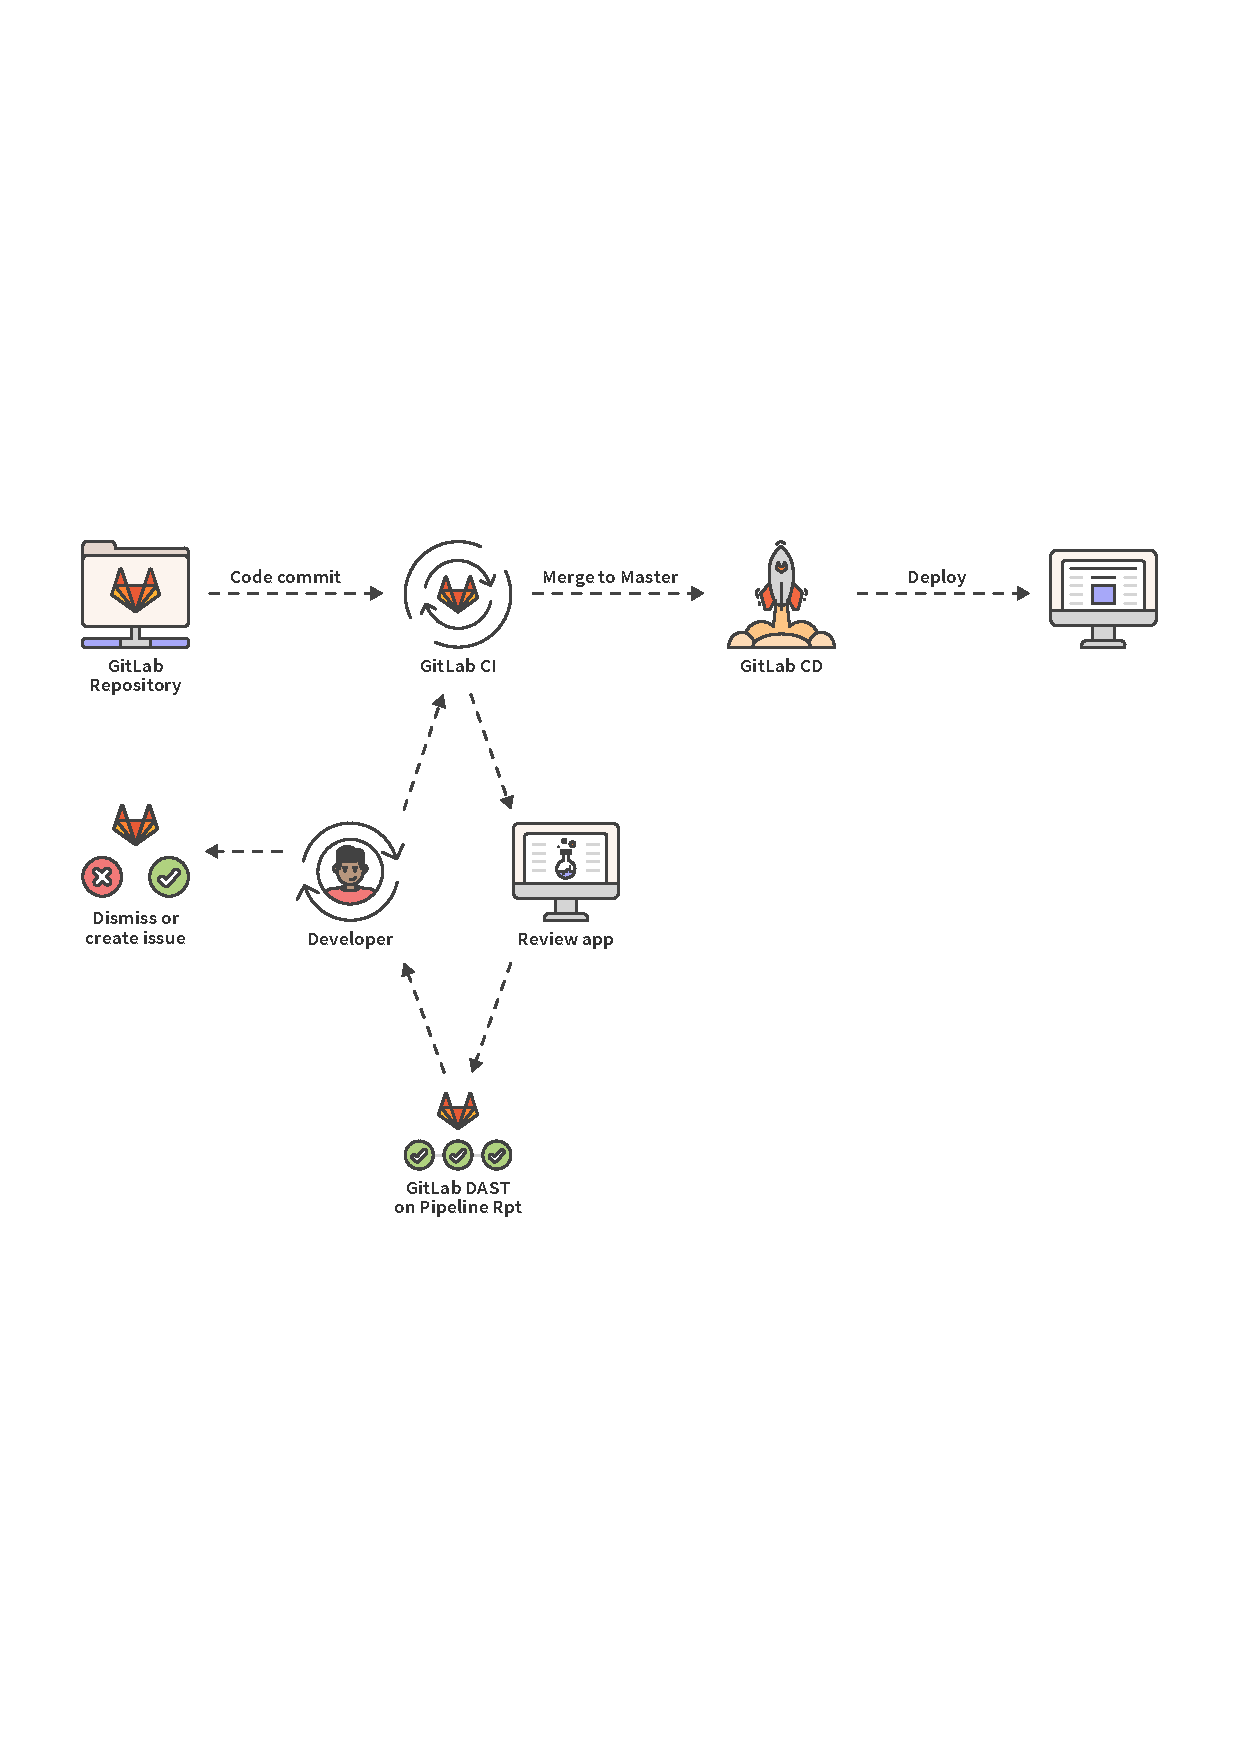
\includegraphics[width=\textwidth]{media/gitlab-review-cycle.pdf}
            \caption{Cyklus kontroly kvality aplikace GitLab s integrovaným \glstext{DAST} \cite{gitlab-app-security}. Vývojář může vyhodnotit bezpečnostní problémy před začleněním změň do sdíleného kódu.}
            \label{fig:gitlab-review-cycle}
        \end{figure}

        \todo{Jaké jsou historická CVE? Jaká je izolace klientů? Co aplikace potřebuje za přístupy?}\blind[1]

    \subsection{Dostupnost}
        \subsubsection{GitLab omnibus}
            Omnibus distribuce GitLabu, tedy balíček který obsahuje všechny komponenty, je primárně pro snadné nasazení a nepočítá se s tím, že by běžel s vysokou dostupností (\HA). Umožňují ale aktualizovat systém bez výpadku: doporučený postup je aktualizovat balíček, spustit databázové migrace a reloadnout webový frontend a konzumenty fronty \cite{gitlab-omnibus-update}. Důsledně se snaží dodržovat kompatibilitu napříč verzemi a databázové migrace dělají zpětně kompatibilní. V každém vydání nové verze jsou změny rozepsané a případné nekompatibility jsou znárorněny v tzv. \textit{upgrade barometer}.

            V základním nastavení nelze GitLab Omnibus replikovat. Některé komponenty lze ale vyčlenit. Nezbytné jsou PostgreSQL a Redis. Jediné co pak zbývá a sdílí se mezi replikami jsou samotné git repozitáře na souborovém úložišti. Vyzkoušel jsem, že GitLab Omnibus správně funguje ve víc replikách, když se vyčlení databáze a repozitáře se sdílí přes \glstext{NFS}. Jedná se ale o nezdokumentované nasazení a nemá oficiální podporu.

            Při nasazení ve víc replikách lze docílit 100 \% dostupnosti při aktualizaci na novější verzi.

        \subsection{GitLab microservices}
            \todo{todo popsat: vypsat komponenty a pak sepsat ze gitaly neni HA}

        \todo{Může gitlab běžet ve víc replikách? Jak se dělá upgrade? Jak stabilní to je?}\blind[2]

    \subsection{Integrace}
        \todo{Integrace gitlabu, oznámení na GitHub/GitLab/Bitbucket/\ldots}\blind[2]
        \todo{Možnosti deploy z gitlabu do cílového systému; k8s, sftp, openstack, \ldots}\blind[5]

    \subsection{Praktické nasazení projektů}
        \subsubsection{Projekt 1}
            \todo{Popsat deploy projektu 1 z gitlabu}\blind[2]
        \subsubsection{Projekt 2}
            \todo{Popsat deploy projektu 2 z gitlabu}\blind[2]
        \subsubsection{Projekt 3}
            \todo{Popsat deploy projektu 3 z gitlabu}\blind[2]
            \todo{popsat že to má docker registry, že shell executor je rychlý protože sdílí cache, ale naprd protože sdílí credentials a image}
